\begin{tikzpicture}[cap=round]
\begin{axis}[
    % temporary
    width=0.9\textwidth,
    height=0.4\textwidth,
    ylabel={$t$ [s]},
    xlabel={number of basis functions $N$ [--]},
    legend pos=north west,
    legend style={font=\small, xshift=-2mm},
    grid=major,
    xminorgrids,
    grid style={dashed},
    xmode=log,
    ymode=log,
    smooth,
    xmin=99,
    xmax=9999
]
    % non-accelerated
    \addplot[
        mark options={scale=0.3, fill=PairedA},
        color=PairedF,
        line width=0.5mm,
    ] coordinates {
        (99.000000, 0.158007)
        (199.000000, 0.668733)
        (299.000000, 1.686584)
        (399.000000, 2.610131)
        (499.000000, 4.528961)
        (599.000000, 6.671688)
        (699.000000, 8.639862)
        (799.000000, 11.236088)
        (899.000000, 13.846618)
        (999.000000, 16.432553)
        (1099.000000, 19.298922)
        (1199.000000, 22.405018)
        (1299.000000, 26.892712)
        (1399.000000, 30.497404)
        (1499.000000, 34.862480)
        (1599.000000, 39.501284)
        (1699.000000, 44.402851)
        (1799.000000, 48.343023)
        (1899.000000, 52.147783)
        (1999.000000, 55.727684)
        (2099.000000, 61.240145)
        (2199.000000, 66.487483)
        (2299.000000, 73.025356)
        (2399.000000, 80.128868)
        (2499.000000, 86.713613)
        (2599.000000, 92.246507)
        (2699.000000, 98.534262)
        (2799.000000, 107.105024)
        (2899.000000, 140.515509)
        (2999.000000, 175.151825)
        (3099.000000, 164.001858)
        (3199.000000, 181.756651)
        (3299.000000, 194.967335)
        (3399.000000, 204.363800)
    };

    % interaction symmetries acceleration worst case scenario
    \addplot[
        name path=wc,
        mark options={solid, scale=0.3, fill=PairedC},
        color=PairedD,
        line width=0.5mm,
    ] coordinates {
        (100.000000, 0.008455)
        (199.000000, 0.018150)
        (301.000000, 0.026514)
        (400.000000, 0.041772)
        (500.000000, 0.057923)
        (601.000000, 0.072488)
        (700.000000, 0.095966)
        (799.000000, 0.127861)
        (901.000000, 0.156602)
        (1000.000000, 0.176823)
        (1100.000000, 0.348475)
        (1200.000000, 0.288771)
        (1300.000000, 0.345407)
        (1399.000000, 0.335197)
        (1501.000000, 0.410222)
        (1600.000000, 0.433115)
        (1700.000000, 0.638818)
        (1800.000000, 0.652821)
        (1900.000000, 0.634285)
        (1999.000000, 0.702872)
        (2101.000000, 0.837659)
        (2200.000000, 0.884804)
        (2300.000000, 1.413141)
        (2401.000000, 1.007031)
        (2500.000000, 1.212241)
        (2600.000000, 1.258247)
        (2700.000000, 1.530978)
        (2800.000000, 1.545223)
        (2899.000000, 1.526760)
        (3000.000000, 1.898381)
        (3100.000000, 1.703769)
        (3200.000000, 2.577140)
        (3300.000000, 2.012791)
        (3400.000000, 2.048295)
        (3499.000000, 2.175623)
        (3600.000000, 2.718274)
        (3700.000000, 2.600659)
        (3800.000000, 3.658818)
        (3900.000000, 4.195028)
        (4000.000000, 4.047160)
        (4100.000000, 5.701685)
        (4200.000000, 5.149829)
        (4300.000000, 4.140006)
        (4400.000000, 5.681671)
        (4501.000000, 4.684606)
        (4600.000000, 5.110454)
        (4700.000000, 5.473549)
        (4801.000000, 5.563717)
        (4900.000000, 4.813465)
        (5000.000000, 9.313194)
        (5100.000000, 10.174398)
        (5200.000000, 5.994061)
        (5299.000000, 6.456540)
        (5400.000000, 6.773736)
        (5500.000000, 6.963583)
        (5600.000000, 8.389064)
        (5700.000000, 8.231182)
        (5800.000000, 7.913203)
        (5899.000000, 7.867099)
        (6000.000000, 8.688807)
        (6100.000000, 8.672424)
        (6199.000000, 9.504774)
        (6301.000000, 9.623434)
        (6400.000000, 9.912002)
        (6499.000000, 10.179926)
        (6600.000000, 12.834426)
        (6700.000000, 10.433521)
        (6800.000000, 11.060281)
        (6900.000000, 13.848520)
        (7000.000000, 11.244264)
        (7100.000000, 12.440672)
        (7201.000000, 11.652530)
        (7300.000000, 12.260372)
        (7400.000000, 15.705102)
        (7500.000000, 13.055222)
        (7600.000000, 13.151486)
        (7699.000000, 13.537049)
        (7801.000000, 15.871871)
        (7900.000000, 14.391479)
        (7999.000000, 15.262016)
        (8100.000000, 18.010433)
        (8200.000000, 14.262222)
        (8300.000000, 14.646533)
        (8400.000000, 17.884314)
        (8500.000000, 14.175818)
        (8600.000000, 20.710682)
        (8701.000000, 15.161741)
        (8800.000000, 14.949150)
        (8900.000000, 16.372537)
        (9000.000000, 20.005114)
        (9100.000000, 16.423370)
        (9199.000000, 16.510193)
        (9300.000000, 18.037983)
        (9400.000000, 17.523011)
        (9499.000000, 19.537410)
        (9600.000000, 19.024318)
        (9700.000000, 19.202945)
        (9800.000000, 23.432156)
        (9901.000000, 19.904437)
        (9999.000000, 21.289400)
    };

    % interaction symmetries acceleration best case scenario
    \addplot[
        name path=bc,
        mark options={scale=0.3, fill=PairedA},
        color=PairedB,
        line width=0.5mm,
    ] coordinates {
        (99.000000, 0.004414)
        (199.000000, 0.009740)
        (299.000000, 0.013137)
        (399.000000, 0.020226)
        (499.000000, 0.023924)
        (599.000000, 0.031702)
        (699.000000, 0.041319)
        (799.000000, 0.051255)
        (899.000000, 0.061279)
        (999.000000, 0.073340)
        (1099.000000, 0.084757)
        (1199.000000, 0.104490)
        (1299.000000, 0.125388)
        (1399.000000, 0.133127)
        (1499.000000, 0.154151)
        (1599.000000, 0.155299)
        (1699.000000, 0.189041)
        (1799.000000, 0.212779)
        (1899.000000, 0.230527)
        (1999.000000, 0.261444)
        (2099.000000, 0.288493)
        (2199.000000, 0.327777)
        (2299.000000, 0.347811)
        (2399.000000, 0.370857)
        (2499.000000, 0.406255)
        (2599.000000, 0.428323)
        (2699.000000, 0.484185)
        (2799.000000, 0.495719)
        (2899.000000, 0.568444)
        (2999.000000, 0.587027)
        (3099.000000, 0.633957)
        (3199.000000, 0.712276)
        (3299.000000, 0.696564)
        (3399.000000, 0.734362)
        (3499.000000, 0.778049)
        (3599.000000, 0.816023)
        (3699.000000, 0.914760)
        (3799.000000, 1.110862)
        (3899.000000, 1.141005)
        (3999.000000, 1.451585)
        (4099.000000, 1.315985)
        (4199.000000, 1.409787)
        (4299.000000, 1.524957)
        (4399.000000, 1.639671)
        (4499.000000, 1.750538)
        (4599.000000, 1.824669)
        (4699.000000, 1.935874)
        (4799.000000, 2.058130)
        (4899.000000, 1.836156)
        (4999.000000, 2.200709)
        (5099.000000, 2.052056)
        (5199.000000, 1.968430)
        (5299.000000, 2.058741)
        (5399.000000, 2.151720)
        (5499.000000, 2.232796)
        (5599.000000, 2.277467)
        (5699.000000, 2.393735)
        (5799.000000, 2.526778)
        (5899.000000, 2.524227)
        (5999.000000, 2.747404)
        (6099.000000, 2.748938)
        (6199.000000, 2.793888)
        (6299.000000, 2.866725)
        (6399.000000, 2.990725)
        (6499.000000, 3.192862)
        (6599.000000, 3.162656)
        (6699.000000, 3.217060)
        (6799.000000, 3.332295)
        (6899.000000, 3.445346)
        (6999.000000, 3.616876)
        (7099.000000, 3.750739)
        (7199.000000, 3.799390)
        (7299.000000, 3.857703)
        (7399.000000, 4.280826)
        (7499.000000, 4.072775)
        (7599.000000, 4.060106)
        (7699.000000, 4.272606)
        (7799.000000, 5.156184)
        (7899.000000, 4.527195)
        (7999.000000, 4.760274)
        (8099.000000, 4.603873)
        (8199.000000, 4.688200)
        (8299.000000, 4.186401)
        (8399.000000, 4.404111)
        (8499.000000, 4.534623)
        (8599.000000, 4.526370)
        (8699.000000, 4.757164)
        (8799.000000, 4.879770)
        (8899.000000, 5.025295)
        (8999.000000, 5.148618)
        (9099.000000, 5.340343)
        (9199.000000, 5.659856)
        (9299.000000, 5.638036)
        (9399.000000, 5.866368)
        (9499.000000, 6.125484)
        (9599.000000, 6.121542)
        (9699.000000, 6.504247)
        (9799.000000, 6.874297)
        (9899.000000, 6.616012)
        (9999.000000, 7.174892)
    };

    \addplot[
        fill=PairedA,
        draw=none
    ] fill between[
        of=wc and bc,
    ];

    \legend{non-accelerated, accelerated (WC\footnotemark[1]), accelerated (BC\footnotemark[1])}

    % draw an arrow from A to B
    \draw[->, thick, black]
    (axis cs:2.7e2,1e-1) -- (axis cs:1e3,3e-1);

    \node[
      inner sep=0pt,        % no extra padding
      transform shape        % ensure the node itself isn’t scaled by the axis
    ]
    at (axis cs:5e3,2e-2)    % this coordinate *is* log-transformed
    {
\includegraphics[width=2.5cm]{images/dipole_mesh.pdf}};

    \draw[->, thick, black]
    (axis cs:5e3,4e-2) -- (axis cs:3e3,4e-1);

    \node[
      inner sep=0pt,        % no extra padding
      transform shape        % ensure the node itself isn’t scaled by the axis
    ]
    at (axis cs:2.2e2,1e-1)    % this coordinate *is* log-transformed
    {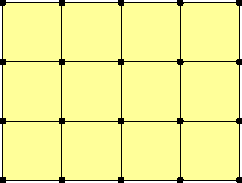
\includegraphics[width=0.7cm]{images/rect_mesh.pdf}};
\end{axis}
\end{tikzpicture}
